\documentclass[spanish,a4paper,11pt]{report}
%%%%%%%%%%%%%%%%%%%%%%%%%%%%%%%%%%%%%%%%%%%%%%%%%%%%%%%%%%%%%%%%%%%%%%%%%%%%%%%
\usepackage{graphicx}
\usepackage{epsfig}
\usepackage[spanish]{babel}
\usepackage[utf8]{inputenc}
\usepackage[dvipdfm]{hyperref}


\begin{document}

\pagestyle{empty}
\thispagestyle{empty}

\newcommand{\HRule}{\rule{\linewidth}{1mm}}
\setlength{\parindent}{0mm}
\setlength{\parskip}{0mm}
\vspace*{\stretch{1}}


\HRule
\begin{center}
        {\Huge \bf Integración Simpson} \\[2.5mm] 
        {\Huge \Large \[f(x) = \frac{x^3}{1+x^\frac{1}{2}}, x \in [1,2]\]} \\[2.5mm]
        {\Large Lorena Morales Pérez\\[2mm]
                Ashneet Khandpur Singh\\[2mm]
                Cristina González Marrero}\\[5mm]
        {\Large \textit{Grupo 2 }} \\[5mm]


        {\em Técnicas Experimentales. $1^{er}$ curso. $2^{do}$ semestre} \\[5mm]
        Lenguajes y Sistemas Informáticos \\[5mm]
        Facultad de Matemáticas \\[5mm]
        
        Universidad de La Laguna \\
\end{center}
\HRule
\vspace*{\stretch{2}}
\begin{center}
  La Laguna, \today 
\end{center}


\newpage

\begin{abstract}

\parindent=1cm Sabemos que una integral definida se define geométricamente como el área bajo la curva f(x) en el intervalo[a,b].
Desafortunadamente en la mayoría de los casos prácticos es muy difícil hallar una antiderivada de f(x). En estos casos el valor
de la integral debe aproximarse. Existen varias maneras para ello, por modelos ó métodos numéricos, aplicar la regla Trapezoidal 
o Rectangular con segmentos cada vez más pequeños o bien, utilizar las Reglas de SIMPSON aplicando polinomios de orden superior
para conectar los puntos, con la cual se obtiene una estimación más exacta de una integral. Por ejemplo si hay un punto medio 
extra entre f(a) y f(b), entonces se puede conectar los tres puntos con una parábola. Dicho de otra manera, para cada aplicación 
de la regla de SIMPSON se requieren dos subintervalos, a fin de aplicarla N número de veces, deberá dividirse el intervalo 
(a,b) en un número de subintervalos o segmentos. Cada subintervalo sucesivo se aproxima por un polinomio de segundo grado 
(parábola) y se integra de tal manera que la suma de las áreas de cada segmento de la parábola sea la aproximación a la 
integración deseada, como veremos a lo largo del proyecto.

\end{abstract}


\tableofcontents

\newpage{\pagestyle{empty}\cleardoublepage}

\renewcommand{\thepage}{\arabic{page}}
\setcounter{page}{1}

\setlength{\parindent}{5mm}

\chapter{Motivación y objetivos}

\section{Objetivo General}
\label{chapter:obj}

\parindent=1cm Nuestro principal objetivo en este proyecto de investigación, es comprender el funcionamiento del método de 
simpson aplicado a nuestra funcion expuesta en la portada, asi como acotar el error cometido en la integración numérica a través de éste.

\parindent=1cm De manera general, queremos saber: 
Resolver el problema de cálculo del área bajo la curva entre dos límites conocidos, dividiendo en N subáreas para calcular 
su valor, asumiendo cada subárea como un pequeño arco de parábola. 
Comprender las bases conceptuales de la integración aproximada,
comprender los rasgos generales de la integración aproximada utilizando el método de Simpson,
comprender la aproximación del error por truncamiento de la integración aproximada utilizando el método de Simpson, frente al 
valor exacto y resolver problemas de integración numérica, utilizando el método de Simpson.





\section{Objetivo Específico}
\label{chapter:espec}

\parindent=1cm Entrando más en detalle, realizamos el trabajo para:  

\begin{itemize}
  \item Conocer la interpretación geométrica de la integral definida
  \item Reconocer que el método de Simpson representa, geométricamente, el área bajo una función polinomial de segundo orden 
  (Cuadrática o Parabólica).
  \item Acotar el error cometido en la integración numérica por el método de Simpson.
  \item Explicar la obtención de fórmulas más precisas para calcular,numéricamente, integrales definidas.
  \item Aplicar el método de Simpson, para calcular numéricamente, las aproximaciones de algunas integrales definidas.
\end{itemize}

\begin{figure}[ptb]
\begin{center}
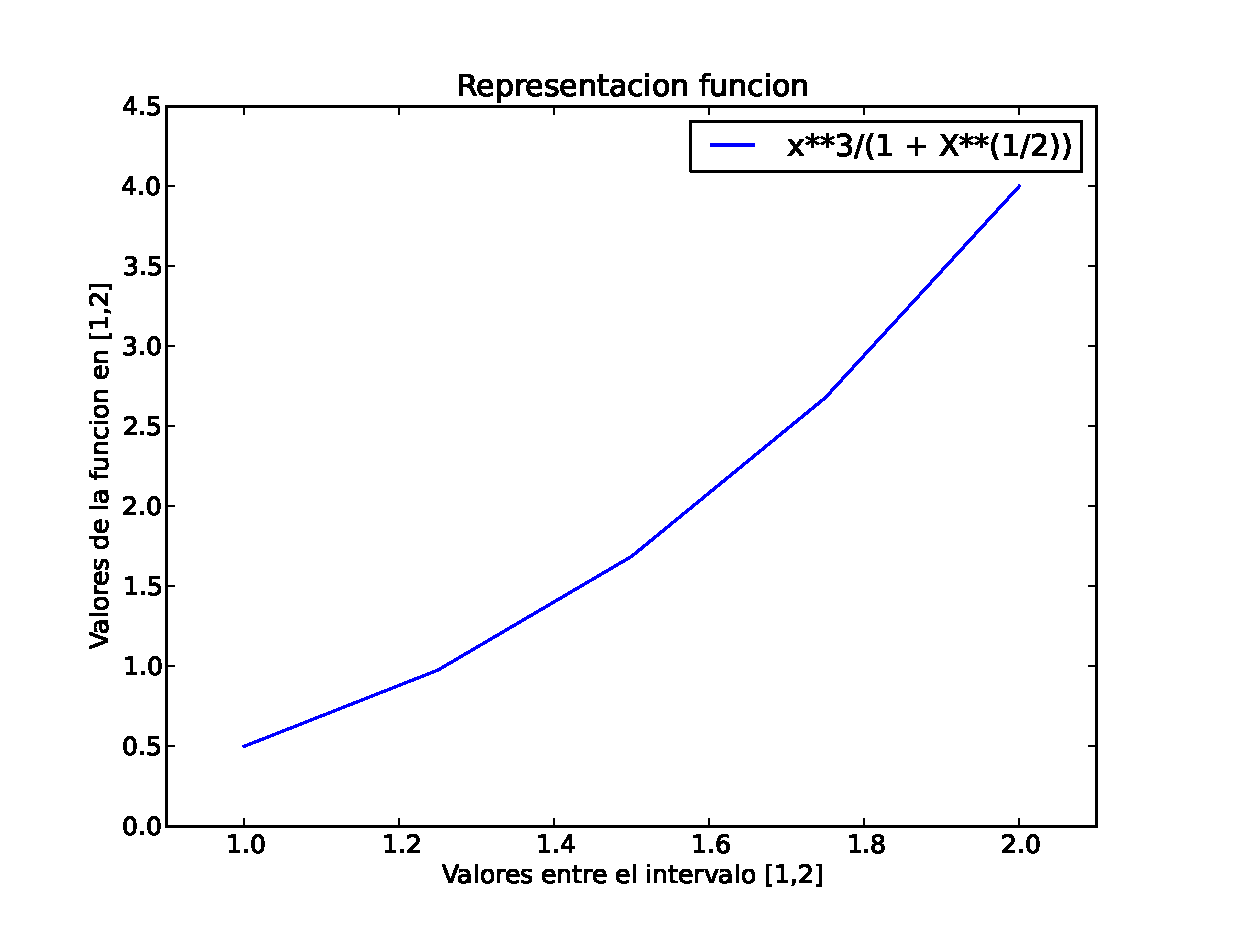
\includegraphics[width=0.75\textwidth]{tmp2.eps}
\caption{Gráfica de la función}
\label{fig:1}
\end{center}
\end{figure}


\chapter{Fundamentos Teóricos}


\section{Antecedentes Teóricos}   
\label{chapter:teo}

\parindent=1cm En análisis numérico, la regla o método de Simpson (nombrada así en honor de Thomas Simpson) y a veces llamada 
regla de Kepler es un método de integración numérica que se utiliza para obtener la aproximación de la integral:

\[\int_a^{b}f(x) \: dx \approx \frac{b-a}{6} \Bigg[f(a)+4f\Big(\frac{a+b}{2}\Big)+f(b)\Bigg]\]


Además se puede determinar que la ecuación anterior tiene un error asociado de:

\[E_t = \frac{-1}{90}h^5 f^4(\xi)\]

La expresión anterior se puede expresar también así:

\[E_t = -\frac{(b-a)^5}{2880}f^4(\xi)\]

El término \[f^4(\xi)\] lo podemos  aproximar al promedio de la cuarta derivada.

\[i^4(\xi) = \frac{\int_a^{b} i^4 (\lambda)d\lambda }{b-a}\]

El error asociado a la regla de Simpson nos indica que este método es más exacto que otros métodos de integración como la regla 
del trapecio. Vemos que el error es proporcional a la cuarta derivada, por lo tanto el coeficiente del tercer grado se hace cero 
en la interpolación polinomial. Esto quiere decir que para ecuaciones de tercer grado se obtienen ecuaciones exactas aunque se 
aproxime con una parábola. Así, el método de Simpson es muy relevante.


En el caso de que el intervalo [a,b] no sea lo suficientemente pequeño, el error al calcular la integral puede ser muy grande. 
Para ello, se recurre a la fórmula compuesta de Simpson. Se divide el intervalo [a,b] en N subintervalos iguales (con n par)

\[\int_a^{b}f(x) \: dx \approx \frac{h}{3} \Bigg[f(x_o)+ 2\Sigma_{j=1}^{n/2-1} f(x_2j) + 4\Sigma_{j=1}^{n/2} f(x_2j-1) + f(x_n)\Bigg]\]

Por último, hablaremos de un poco de historia de este método en el apéndice final.

\section{Antecedentes Prácticos}   
\label{chapter:pra}

Para la resolución del problema ya citado, se ha utilizado python ya que es útil para estudiar este tipo de problemas debido a 
que permite la inclusión de representaciones gŕaficas. 
Python es un lenguaje de programación creado por Guidon van Rossum a principios de los años 90, cuyo nombre está inspirado en 
el grupo de los cómicos ingleses "Monty Python". Se trata de un lenguaje de programación interpretado, es decir, aquel que se 
ejecuta usando otro programa denominado intérprete, en lugar de compilar el código a lenguaje máquina y permitir que el odenador 
lo pueda entender y ejecutar directamente. Con esto último se hace referencia al lenguaje compilado, en el que la ejecución es
mas rápida que en los lenujajes interpretados,aunque éstos son más flexibles y portables. 
Python tiene la característica de ser dinámico, lo que quiere decir que no es necesario declarar el tipo de dato que va a 
contener una determinada variable, ya que viene determinado según el valor que se le asigne, teniendo en cuenta que el tipo 
puede cambiar si se le asigna otro valor de otro tipo diferente ,al contrario que en el lenguaje de programación C.
  
\parindent=1cm Además, Python es fuertemente tipado, lo que quiere decir que no se permite tratar a una variable como si fuera
de un tipo distinto al que tiene. Debemos saber que está disponible en múltiples plataformas, como UNIX, Windows, Mac OS, etc 
(multiplataforma).
También cabe destacar que los programas realizados con Python parecen pseudocódigo (lenguaje similar al nuestro) y por ello se 
considera de alto nivel.
Finalmente, es importante añadir que la indentación es muy importante para la correcta ejecución de estos.
  

\chapter{Procedimiento experimental}

\section{Descripción de los experimentos}    
\label{chapter:exp} 

Como ya se ha mencionado, para resolver nuestro problema del cálculo aproximado de la integral de una función mediante la Regla 
de Simpson, se ha utilizado el lenguaje de programación Python.
El objetivo es, utilizando la fórmula simple y compuesta de la regla de Simpson, calcular una aproximación de la integral. Durante
el desarrollo de los experimentos se ha mostrado interés por conocer el error de dicha aproximación, al igual que el tiempo que tarda nuestra computadora en realizar este cálculo.\par
En primer lugar, durante el desarrollo del programa, se ha creado un subrograma que se encarga en de calcular la aproximación de
la integral mediante la fórmula simple. Como ya se ha comentado, nos interesa también saber el error que se obtiene al calcular 
esta aproximación. Para ello, tras haber creado una constante con el valor exacto de la integral en el programa principal, se obtiene
el error mediante la resta de la aproximación menos la integral. Ya que también estamos interesados en conocer el tiempo que tarda
Python en calcular esta aproximación, escribimos una función propia del programa que estamos utilizando y nos devuelve el tiempo
transcurrido hasta el momento. Al añadir este comando al final del subprograma, se calcula el tiempo que tarda la máquina después 
de realizar el cálculo de aproximación de la integral. Por tanto, al restar los valores del tiempo obtenidos al inicio y al fin 
del subprograma, se obtiene el tiempo total invertido en este procedimiento. Como es lógico, esta función devolvería la aproximación
de la integral, el error y el tiempo que tarda en realizar dicho cálculo.\parindent=1cm
El experimento se ha seguido con otro subprograma que se encarga de hacer lo mismo que el anterior pero utilizando la fórmula 
compuesta del método de Simpson. Durante este procedimiento también se ha calculado el error cometido y el tiempo que tarda el 
programa. Como ya sabemos, la fórmula compuesta se diferencia de la simple en que, con esta se puede obtener una 
aproximación no muy acertada y por ello se subdivide el intervalo en el que estamos calculando el área por debajo de la función y
así obtener un margen de error menor. 
Finalmente, se han creado dos subprogramas diferentes en los que se hace la representación de la función que estamos estudiando y,
por otro lado, las representaciones gráficas del error obtenido y el tiempo invertido en el cálculo del valor aproximado de la 
integral. En las gráficas del error y del tiempo obtenido se han empleado los diferentes valores de N, con el objetivo de 
visualizar alguna relación entre el número de subintervalos escogidos y el error y el tiempo obtenidos.


\section{Descripción del material}   
\label{chapter:mat}

El material utilizado para el desarrollo del experimento es el siguiente:

\begin{center}
\begin{footnotesize}
\begin{verbatim}
##########################################################################
#
# CPU Type: Intel(R) Core(TM) i3-2350M CPU @ 2.30GHz
# Cache size: 6144 KB
# CPU speed: 2267.448 Hz
# vendor ID: GenuineIntel
# Name :('Linux','Linux','3.5.0-17-generic','#28-Ubuntu SMP Tue Oct 9 19:31:23 
	   UTC 2012','x86_64','x86_64')
# Platform: Linux-3.5.0-17-generic-x86_64-with-LinuxMint-14-nadia
# Version: 2.7.3
#   
##########################################################################
\end{verbatim}
\end{footnotesize}
\end{center}

\newpage

\section{Resultados obtenidos} 
\label{chapter:result}

Tras implementar nuestro programa en Python, se han obtenido los siguientes resultado:  \parindent=2cm

\begin{figure}[h]
\begin{center}
\begin{tabular}{||c|c c c||} 
 
 \hline
 \hline
 N & Integral & Error & Tiempo \\ 
 \hline
 10 & 1.2672 & -0.3798 & 0.00117 \\
 100 & 1.3044 & -0.3426 & 0.00503 \\
 1000 & 1.3082 & -0.3388 & 0.1333 \\
 10000 & 1.3086 & -0.3384 & 1.1772 \\
 100000 & 1.3086 & -0.3384 & 11.8899 \\
 \hline
 \hline
 
\end{tabular}
\end{center}
\end{figure}

\begin{figure}[h]
\begin{center}
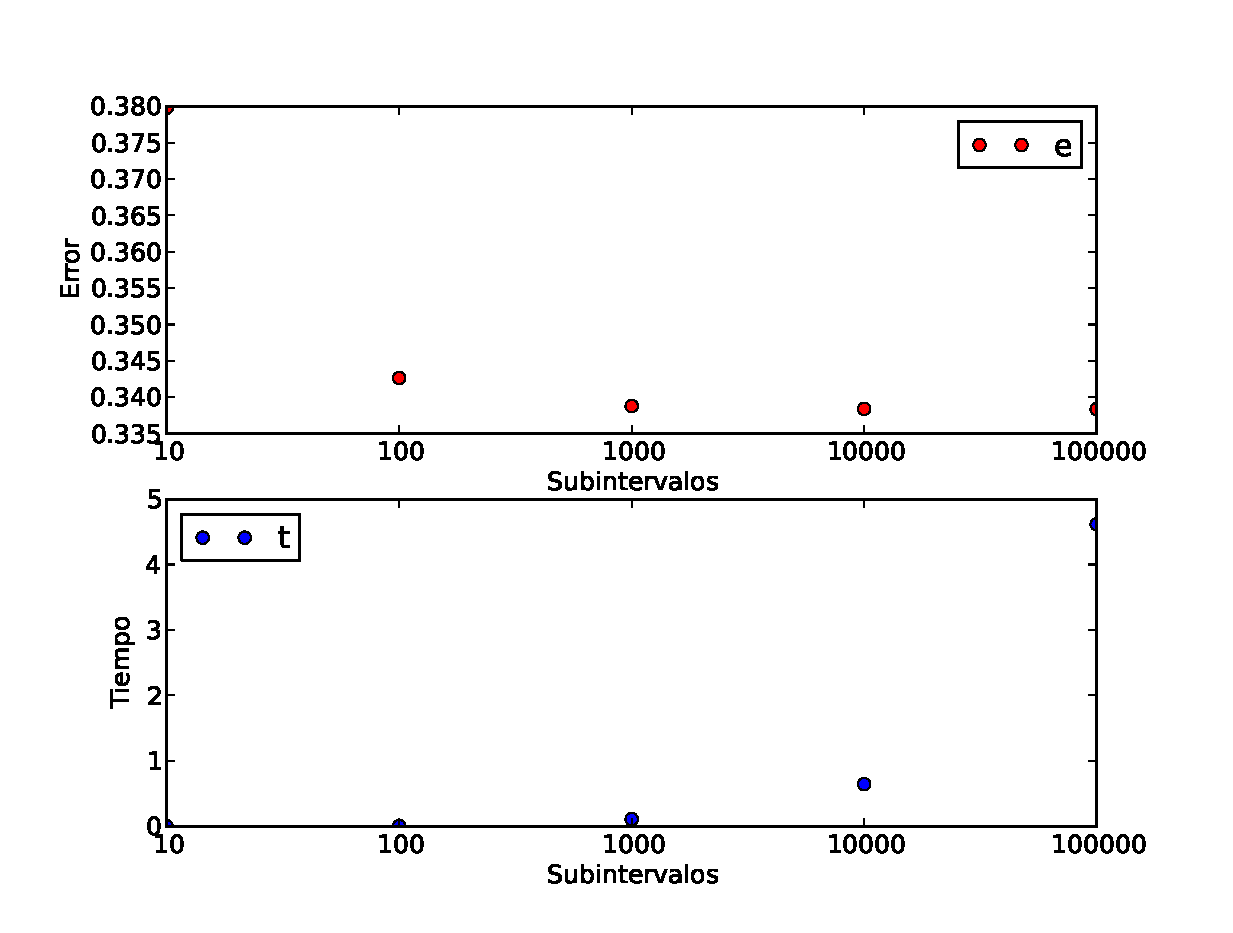
\includegraphics[width=0.75\textwidth]{errortiemp.eps}
\caption{Gráfica del error y tiempo}
\label{fig:2}
\end{center}
\end{figure}

\newpage

\section{Análisis de los resultados}     
\label{chapter:analisis}

Se puede observar en los resultados obtenidos que, cuanto mayor es el valor de N (número de subintervalos en la fórmula compuesta),
menor es el error del cálculo aproximado de la integral. Aunque, en la gráfica situada más abajo se puede comprobar mejor 
este hecho. \par
De la misma manera, se puede observar que el tiempo transcurrido durante el procedimiento de aproximación de la integral 
propuesta, va creciendo según crece el número de subintervalos elegidos. 


\chapter{Conclusiones}
\label{chapter:concl}

\parindent=1cm Como ya sabiamos, la integración numérica consiste en encontrar una buena aproximación al área bajo la curva que representa una 
función f(x), que ha sido determinada a partir de datos experimentales o a partir de una expresión matemática.
Las fórmulas de cuadratura de Newton-Cotes son los procedimientos más comunes de integración numérica; se basan en la estrategia 
de reemplazar una función complicada o datos tabulados con una función aproximada que sea fácil de integrar.  
Estas fórmulas son:

La regla de integración Trapezoidal. \parindent=1cm 
La regla de Simpson.

\parindent=1cm Estas reglas están diseñadas para casos en los que los datos por integrarse están espaciados de manera uniforme. Una forma de 
obtener una aproximación adecuada de una integral es usar polinomios de grado superior para unir los puntos y aproximar la 
función real.
El método de Simpson, a diferencia de la Regla trapezoidal, intenta no incurrir en un mayor número de subdivisiones; se trata 
de ajustar una curva de orden superior en lugar de una línea recta como en la Regla Trapezoidal.

\parindent=1cm En conclusión, la regla de Simpson para el cálculo de integrales es muy apropiada, pero sobretodo el empleo de la fórmula 
compuesta, ya que nos permite elegir el número subintervalos y calcular la integral en cada uno de ellos, de manera que se 
obtiene un valos bastante aproximado de la integral. Aunque, debemos tener en cuenta que cuánto mayor es el número de intervalos,
más tarda el programa en realizar el cálculo. 

\newpage{\pagestyle{empty}\cleardoublepage}
\thispagestyle{empty}

\begin{appendix}

\chapter{Apéndice 1}
\label{appendix:1}


\section{Código python}
\label{Apendice1:YYY}

\begin{center}
\begin{footnotesize}
\begin{verbatim}
/###################################################################################
 # codigo.py
 ###################################################################################
 # -*- coding: utf-8 -*-
import sys
from matplotlib.pylab import *
import time

def integralsimple(f,a,b, integral):   #Cálculo de la integral simple

  inicio = time.time() #Calcula el tiempo transcurrido hasta el momento
  
  h=(b-a)/2;
  x=a
  fa=eval(f)
  x=b
  fb=eval(f)
  x=a+h
  fab=eval(f)
  ftotal=(fa+fb+4*fab)
  integs=(h/3)*ftotal
  
  fin = time.time()  #Calcula el tiempo transcurrido hasta que finaliza este procedimiento
  errort = integs - integral  #Calcula el error de la aproximación
  tiempot = fin - inicio  #Calcula tiempo total invertido en el procedimiento
  
  return integs, errort, tiempot

def integralcomps(funcion,a,b,n, integral):

  inicial = time.time()  # Mide tiempo inicial
  
  h=(b-a)/(3*n)
  f1=0
  i=1
  while i<=(n-1):
    x=a+h*(2*i)
    f1=f1+eval(funcion)
    i+=1
  f2=0
  k=1
  while k<=n:
    x=a+h*(2*i-1)
    f2=f2+eval(funcion)
    k+=1
  f=2*f1+4*f2
  x=a
  fa=f+eval(funcion)
  x=b
  fb=fa+eval(funcion)
  integc=(h/3)*fb
  
  final = time.time()  #Mide tiempo final, calcula la diferencia final - inicial e imprimir
  error = integc - integral  #Calcula error producido con la aproximación
  tiempo = final - inicial  # Calcula tiempo total
  return integc, error, tiempo

def representacionerrortiempo(funcion, a, b, X, integral):

  # Reserva memoria para los valores de Y
  Ye = zeros(len(X))
  Yt = zeros(len(X))
  
  # Da valores a Y
  for w in range(len(X)):
    integc, error, tiempo = integralcomps(funcion, a, b, X[w], integral)
    Ye[w] = error
    Yt[w] = tiempo
  
  # En una misma figura, se representan dos gráficas 
  figure(1) 
  title('Representacion errores y tiempo')
  
  # Primera gráfica
  subplot(211)
  xlabel('Subintervalos')
  ylabel('Error')
  errorplot, = plot(range(len(X)),Ye,'ro')
  xticks(range(len(X)), X)
  legend([errorplot], ('error'), 'best')
  
  #Segunda gráfica
  subplot(212)
  xlabel('Subintervalos')
  ylabel('Tiempo')
  tiempoplot, = plot(range(len(X)),Yt,'bo')
  xticks(range(len(X)), X)
  legend([tiempoplot], ('tiempo'), 'best')
  
  # Devuelve la gráfica como imagen .eps
  savefig('errortiemp.eps')
  
  #Muestra la gráfica
  show()
  
def representacionfuncion(funcion, a, b):

  # Valores de X y reserva memoria para Y
  X = linspace(a, b, 5)  
  Y = zeros(len(X))   
  
  # Da valores a Y
  for i in xrange(len(X)):
    x=X[i]
    Y[i] = eval(funcion)

  plot(X,Y)
  title('Representacion funcion') 
  xlabel('Valores entre el intervalo [1,2]')
  ylabel('Valores de la funcion en [1,2]')
  legend(['x**3/(1 + X**(1/2))'])
  xlim(0.9, 2.1)
  ylim(0.0, 4.5)
  
  # Devuelve imagen con la gráfica
  savefig('tmp2.eps')
  # Muestra gráfica
  show()
  
if __name__=='__main__':
  if len(sys.argv)==5:
    funcion = sys.argv[1]
    a = float(sys.argv[2])
    b = float(sys.argv[3])
    n = int(sys.argv[4])
    X = [10, 100, 1000, 10000, 100000]
    integral = 1.647
    print "Resultados finales colocados en: (Integral, error, tiempo)"
    print "Cálculo integral mediante fórmula simple:", integralsimple(funcion,a,b, integral)
    print "Cálculo integral mediante fórmula compuesta:", integralcomps(funcion,a,b,n, integral)
    print "Representación gráfica de la función:", representacionfuncion(funcion, a, b)
    print "Representación gráfica de la integral y los errores", representacionerrortiempo(funcion, a, b, X, integral)
    
 ##################################################################################
\end{verbatim}
\end{footnotesize}
\end{center}


\chapter{Apéndice 2}
\label{appendix:2}

\section{Un poco de Historia sobre integración simpson}
\label{Apendice2:label}

La fórmula fue utilizada por primera vez por Evangelista Torricelli, pero debe su nombre al matemático Inglés Thomas Simpson. Corresponde a la regla del tonel que Johannes Kepler ya había formulado en 1615.
Sobre la historia de su surgimiento, Kepler informa en la dedicatoria de su publicación posterior: Después de que la primera esposa de Kepler había muerto en Praga en 1611, Kepler se casó nuevamente - en Linz, donde ahora trabajaba - en 1613. Para la boda compró algunos toneles de vino. Puesto ya el vino en la bodega, el vendedor concurrió con una vara de medir y determinó el contenido para todos los barriles sin pensar o calcular, utilizando un mismo método, consistente en que introducía la punta de metal de la vara de medir a través de la piquera , en diagonal hacia los bordes de ambos fondos y la marca en la piquera arrojaba la medida del volumen del contenido. Kepler se sorprendió con aquello de que una diagonal a través del medio del barril pudiera dar una medida sobre el volumen contenido y puso en duda la exactitud de este método, debido a que, por ejemplo, un barril muy bajo que tuviera una base algo más ancha y por eso un volumen contenido mucho menor podría tener el mismo radio a la vista.

\parindent=1cm A raíz de esto, Kepler formuló en 1615 el escrito Nova Stereometria doliorum vinariorum (Nuevo cálculo del contenido de barriles de vino), en el que buscaba métodos verificables para el cálculo del contenido de los toneles de vino. Uno de estos métodos consistió en aproximar la curvatura del barril por una parábola, dado que los cálculos con ayuda de parábolas ya se podían realizar muy exactamente desde Arquímedes.
Entre otras cosas, Kepler describió en este texto una fórmula para el cálculo de la capacidad (más precisamente, del volumen) de barriles de vino con formas irregulares. Esta fórmula arroja valores exactos para el tronco de la pirámide, la esfera, el paraboloide elíptico, el hiperboloide de una hoja y todas las demás superficies de un cuerpo que pueden ser generadas por secciones planas perpendiculares al eje del cuerpo.


\end{appendix}


\addcontentsline{toc}{chapter}{Bibliografía}
\bibliographystyle{plain}

\bibliography{bib/references}
\nocite{*}



\begin{thebibliography}{11}
\bibitem{label}
www.wikipedia.org
\bibitem{label1}
www.slideshare.net
\bibitem{label2}
www.metodos.fam.cie.uva.es
\bibitem{label3}
Python para todos. Raúl González Duque. Mundo geek. GPL. zootropo en gmail. 
\bibitem{label4}
www.aristarco.com.es
\bibitem{label5}
es.scribd.com
\bibitem{label6}
www.artofproblemsolving.com



\end{thebibliography}

 
\end{document}
